\documentclass[pdflatex, sn-mathphys-num]{beamer}

\usepackage[utf8]{inputenc}
\usepackage[T1]{fontenc}
\usepackage{graphicx}
\usepackage[dvipsnames]{xcolor}
\usepackage{microtype}
\usepackage[sorting=none]{biblatex}
\addbibresource{ref.bib}

\usetheme[numbering=counter, progressbar=frametitle, background=light]{metropolis}
\usecolortheme{spruce}

\renewcommand{\familydefault}{\sfdefault}

\definecolor{primary}{RGB}{88, 24, 69}
\definecolor{secondary}{RGB}{255, 87, 51}

\setbeamercolor{frametitle}{fg=white, bg=primary}
\setbeamercolor{progress bar}{fg=secondary, bg=gray!30}
\setbeamerfont{frametitle}{size=\large, series=\bfseries}
\setbeamerfont{title}{size=\LARGE, series=\bfseries}

\title{How Science Works}
\subtitle{And What Doesn't Work}
\author{Julian Avila}
\institute{Universidad Distrital Francisco José de Caldas}
\date{\today}

\begin{document}

\begin{frame}
	\titlepage
\end{frame}

\begin{frame}{Outline}
	\tableofcontents
\end{frame}

\section{What is the Method for Science?}
\begin{frame}{Scientific Method}
	\textbf{Science is not a linear process.}

	The common Scientific method is an
	oversimplification.

	\begin{figure}
		\centering
		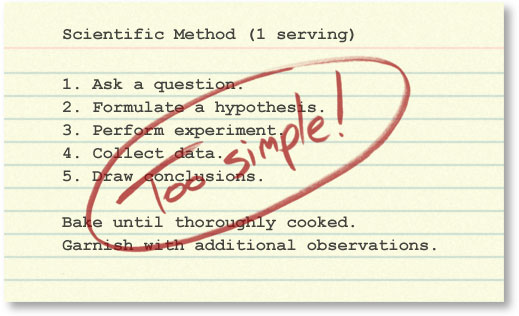
\includegraphics[width=0.7\textwidth]{Figures/sciencerecipe.jpg}
		\caption{The myth of the step-by-step science recipe. \cite{Science}}
	\end{figure}

\end{frame}

\begin{frame}{Then... How Does Science Actually Work?}
	\begin{columns}

		\column{0.6\textwidth}
		\textbf{Science revolves around four interconnected cores:}

		\vspace{0.3cm}
		\begin{itemize}
			\item \textbf{Observation} – Gathering data from the world.
			\item \textbf{Testing} – Evaluating Hypotheses.
			\item \textbf{Feedback} – Refining and adjusting ideas with the Community.
			\item \textbf{Applications} – Using scientific knowledge for Society.
		\end{itemize}

		\column{0.4\textwidth}
		\begin{figure}
			\centering
			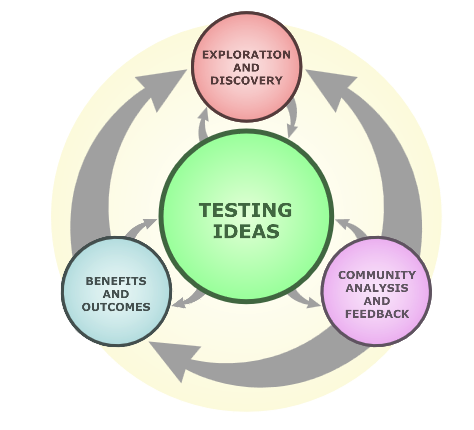
\includegraphics[width=\textwidth]{Figures/canvas.png}
			\caption{Interconnected nature of scientific processes. \cite{Science}}
		\end{figure}

	\end{columns}
\end{frame}

\begin{frame}{The Main Core: Testing Ideas}
	The heart of science is \textbf{testing ideas.}

	Through experimentation and analysis, hypotheses are refined, rejected, or strengthened.
	\begin{figure}
		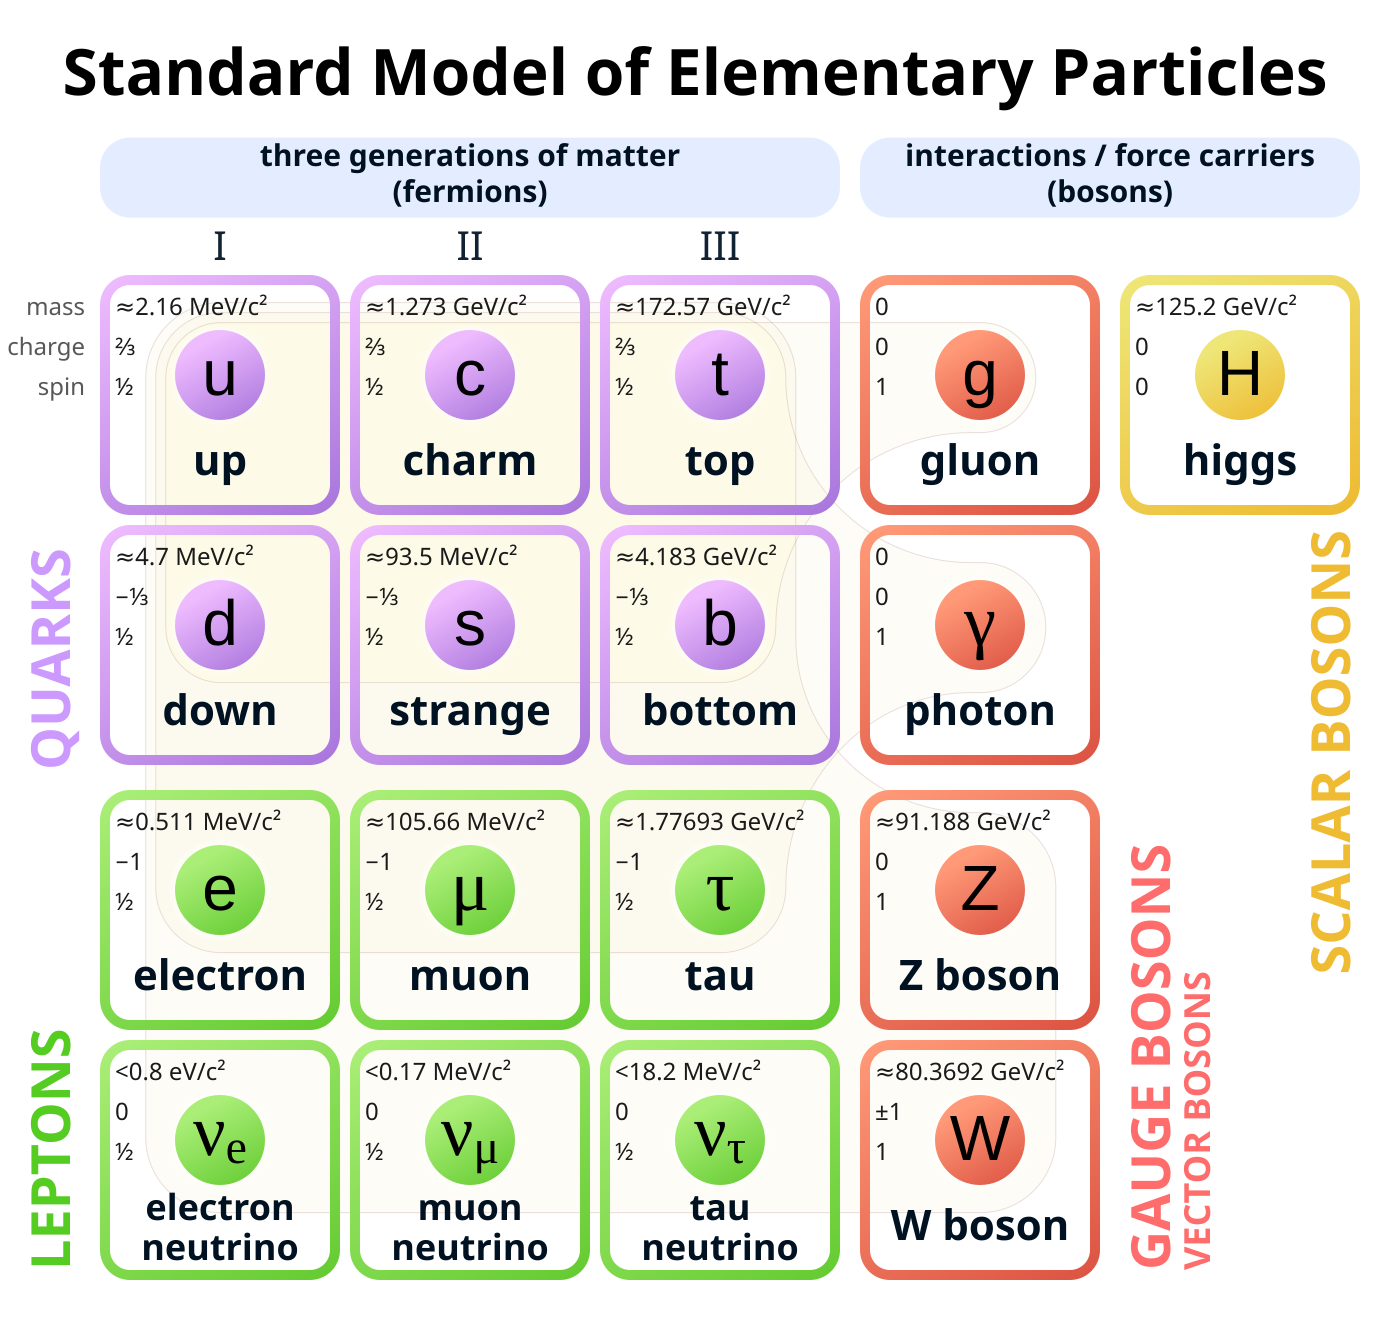
\includegraphics[width=0.5\textwidth]{Figures/Standard-Model.png}
		\caption{Elementary Particles of the Standard Model. \cite{Cush2019}}
	\end{figure}

\end{frame}


\section{Cores of Scientific Method}
\begin{frame}{Observation: Identifying Patterns and Gaps}
  \begin{columns}
    \column{0.5\textwidth}
    \textbf{Processes:}
    \begin{itemize}
      \item Reviewing Scientific Literature
      \item Analysing Known Phenomena
      \item Examining Existing Data
      \item Identifying Unsolved Problems
    \end{itemize}

    \column{0.5\textwidth}
    \textbf{Results \& Connections:}
    \begin{itemize}
      \item Formulation of New Hypotheses
      \item Refinement of Existing Questions
      \vspace{1.81cm}
    \end{itemize}
  \end{columns}
\end{frame}

\begin{frame}{Hypothesis Testing: Validating Scientific Claims}
  \begin{columns}
    \column{0.5\textwidth}
    \textbf{Processes:}
    \begin{itemize}
      \item Designing and Conducting Experiments
      \item Collecting and Analyzing Data
      \item Comparing Results with Predictions
    \end{itemize}

    \column{0.5\textwidth}
    \textbf{Results \& Connections:}
    \begin{itemize}
      \item Discovery of New Patterns or Anomalies
      \item Theory Development or Refinement
      \item Practical Applications in Technology or Industry
    \end{itemize}
  \end{columns}
\end{frame}

\begin{frame}{Peer Feedback: Refining Scientific Knowledge}
  \begin{columns}
    \column{0.5\textwidth}
    \textbf{Processes:}
    \begin{itemize}
      \item Independent Replication of Experiments
      \item Peer Review and Critical Evaluation
      \item Scientific Discussions and Debates
      \item Integration into Theoretical Frameworks
    \end{itemize}

    \column{0.5\textwidth}
    \textbf{Results \& Connections:}
    \begin{itemize}
      \item Identification of Errors or Biases
      \item Generation of New Hypotheses
      \item Expansion of Scientific Applications
      \vspace{1.1cm}
    \end{itemize}
  \end{columns}
\end{frame}

\begin{frame}{Applications: Science in Action}
  \begin{columns}
    \column{0.5\textwidth}
    \textbf{Processes:}
    \begin{itemize}
      \item Development of New Technologies
      \item Implementation in Medicine, Engineering, and Society
      \item Identification of Emerging Challenges
    \end{itemize}

    \column{0.5\textwidth}
    \textbf{Results \& Connections:}
    \begin{itemize}
      \item New Observations for Future Research
      \item Inspiration for Novel Experimental Approaches
      \vspace{1.1cm}
    \end{itemize}
  \end{columns}
\end{frame}


\section{Practical Example}
\include{Sections/practical-example}

\section{Important Facts}
\begin{frame}{Theories Evolve}
  Theories are not set in stone—new evidence refines and improves them 
  over time.

  \vspace{0.5cm}

  \begin{figure}
    \centering
    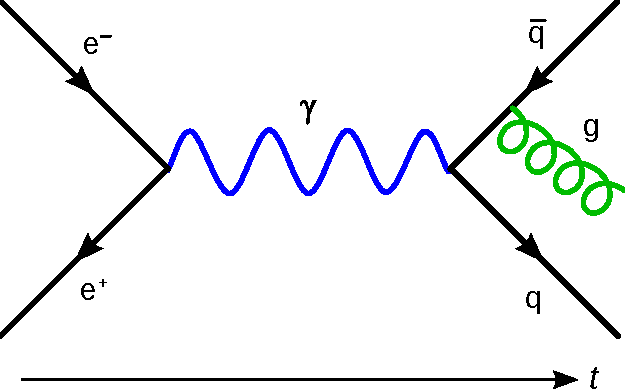
\includegraphics[width=0.7\textwidth]{Figures/Feynmann_Diagram_Gluon_Radiation.pdf}
    \caption{Quantum Field Theory, one of the most successful theories. 
    \cite{Holdsworth2007}}
  \end{figure}
\end{frame}

\begin{frame}{Principle of Parsimony}
  The simplest explanation is preferable.

  \vspace{0.5cm}
  \textbf{Example: Renormalization in Quantum Field Theory}

  Instead of introducing an infinite number of parameters, 
  renormalization allows QFT to explain physical phenomena using 
  only a few experimentally determined constants. 

  \vspace{0.5cm}
  The success of the \textbf{Standard Model} lies in its parsimony: 
  a limited set of symmetries and fundamental interactions describes 
  a vast array of experimental results.
\end{frame}

\begin{frame}{Peer Review is not Absolute}
  While it helps ensure better research, peer review has limitations—
  it can become a barrier to knowledge or create a false sense of quality.

  \vspace{0.5cm}
  \textbf{Example: Reinvention of Calculus in 1994}

  A peer-reviewed medical paper unknowingly reinvented the 
  \textbf{trapezoidal rule} for numerical integration, illustrating how 
  errors can persist in published research. \cite{Tai1994}
\end{frame}

\begin{frame}{Example: Reinvention of Calculus}
  \begin{figure}
    \centering
    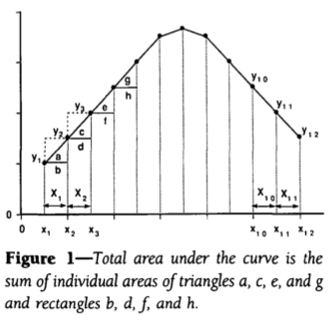
\includegraphics[width=0.7\textwidth]{Figures/calculus.png}
    \vspace{-0.25cm}
    \caption{Taken from paper. \cite{Tai1994}}
  \end{figure}
\end{frame}


\section{Conclusions}
\begin{frame}{\textbf{Conclusion: Questions Drive Research}}

  \onslide<1->{\textbf{RQs and hypotheses} are \alert{crucial} for all research types.}

  \vspace{0.3cm}

  \onslide<2->{They must be developed \textbf{at the start} of the study.}

  \onslide<3->{\emph{Excellent RQs lead to superior hypotheses.}}

  \vspace{0.3cm}

  \onslide<4->{
    \begin{block}{Why They're Important}
      \begin{itemize}
        \item<5-> Guide research direction like a \alert{compass}
        \item<6-> Determine study design, goals, and outcomes
        \item<7-> Prevent ethical and methodological issues
      \end{itemize}
    \end{block}
  }

\end{frame}

\begin{frame}{\textbf{Final Thought}}

  \onslide<1->{The development of RQs and hypotheses is an \alert{iterative process}.}

  \vspace{0.3cm}

  \onslide<2->{It requires:}

  \begin{itemize}
    \item<3-> Deep understanding of the literature
    \item<4-> Insight into the knowledge gap
    \item<5-> Clear, focused, and specific formulation
  \end{itemize}

  \vspace{0.3cm}

  \onslide<6->{\textbf{Plan carefully. Think critically. \emph{Design with purpose.}}}

\end{frame}


\section{Bibliography}
\begin{frame}[allowframebreaks]{Bibliography}
	\printbibliography
\end{frame}

\end{document}
